% 
%  chapter3.tex
%
\chapter{Functional and Non-Functional Requirements}
\label{ch:functionalities}
This chapter details the functional and non-functional requirements and presents a mock \acrfull{ui} that will satisfy the requirement.

The main features of CASCIFFO can be separated into two groups: general functionalities and clinical component.
These two groups contain the functional requirements of CASCIFFO.

This chapter's structure is as follows:

\begin{itemize}
    \item General features - details each of the general features of the platform;
    \item Clinical component features - details each of the clinical component features of the platform;
    \item Non-functional requirements - describes the non-functional requirements.
\end{itemize}

\section{General Features}
\label{sec:general-features}
The general features of CASCIFFO consist in the following:
\begin{itemize}
    \item Visualization and management of Clinical Trials as a process; 
    \item Ability to edit and validate data (edit checks);
    \item Access control based on different user profiles; 
    \item Access by computer, tablet or smartphone; 
    \item Ability to export information in numerical or graphical mode; 
    \item Ability to customize the form of visualization.
\end{itemize}
Each of these features will be detailed in this section.

\subsection{Visualization and Management of Clinical Trials as a Process}
\label{subsec:visualization-clinical-trials-as-process}
To view and manage a clinical trial as a process, a user needs only to view the general overview of Clinical Trials or clinical investigations Proposals.
As in figure~\ref{fig:propostas} and figure~\ref{fig:ensaios}, the user has an overview of the all submitted proposals and clinical trials with their main characteristics, such as, the identification, current state, last alteration date, the principal investigator and whether it has partnerships or not.

\begin{figure}[H]
    \centering
    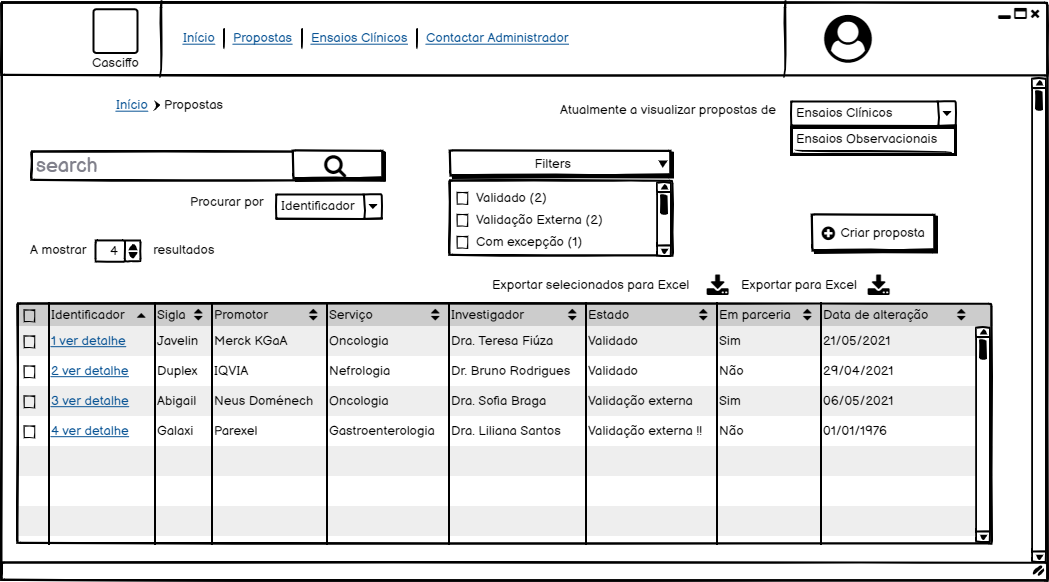
\includegraphics[scale=0.35]{Chapters/img/propostas/proposals.png}
    \caption{Mock overview of clinical investigations proposals.}
    \label{fig:propostas}
\end{figure}

\begin{figure}[H]
    \centering
    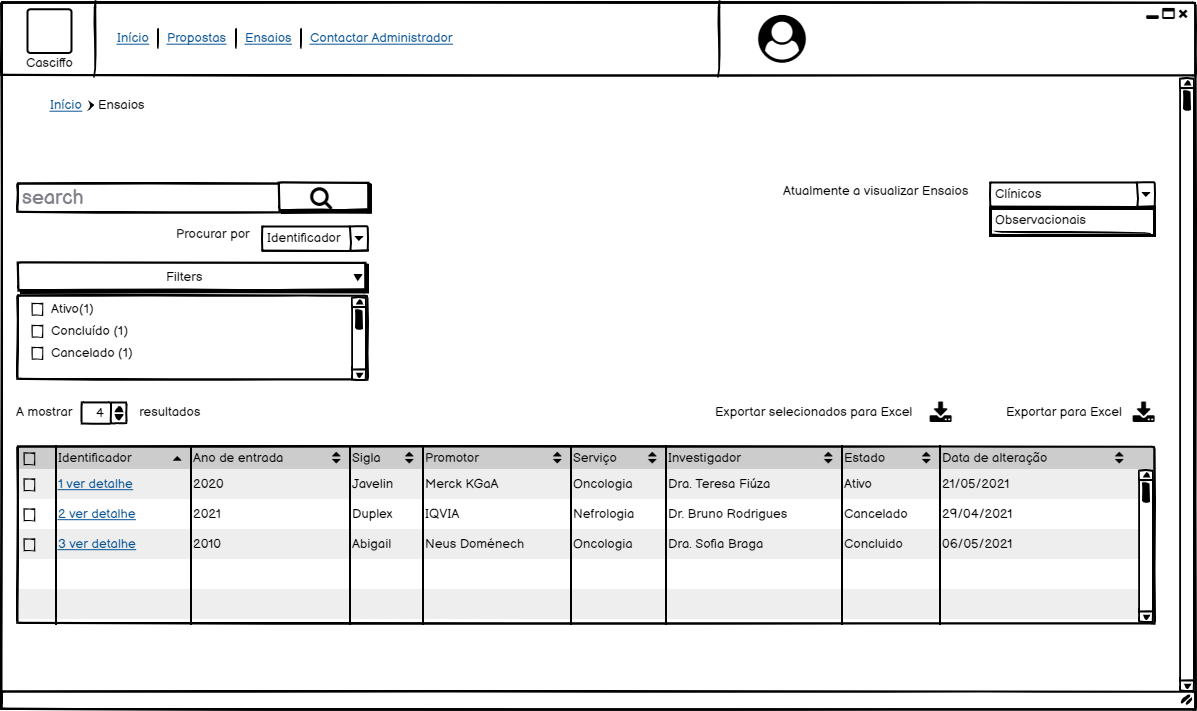
\includegraphics[scale=0.35]{Chapters/img/ensaios/ensaios.png}
    \caption{Mock overview of clinical trials.}
    \label{fig:ensaios}
\end{figure}


When a user clicks the link view details ("ver detalhe"), he will be redirected to a screen displaying the details of the target clinical investigation.

\subsection{Ability to edit and validate data (edit checks)}
\label{subsec:abilitiy-to-edit}
Within the CASCIFFO platform, the \acrshort{uic} and internal departments can view the details of a certain clinical investigation proposal and edit or validate according to their roles.
Users with `\acrshort{uic}` role will be able to create and edit their own Investigations, whereas the internal departments, with roles of `CA`, `Finance` and `Juridical` will only be able to validate the proposals.  
The creation of a proposal starts in the overview of proposals screen, from there a user can click on Create Proposal ("Criar proposta") and will be redirected to the screen illustrated in figure~\ref{fig:criar-proposta}. Here an investigator can choose what type of investigation this proposal corresponds to, either an observational or clinical trial. In the case a clinical trial is selected, more options will be shown since clinical trials have a corresponding financial component.
The data fields corresponding to the therapeutic area, the service and the pathology of an investigation are restricted to a set of possible inputs. In addition, the members of a medical team also belong to an already defined database, being validated at the time of creation of the medical team for the investigation.  
Certain fields cannot be changed once a proposal has been submitted, such as the promoter, the partnerships and the type of investigation can only be defined during the creation of a proposal.  


\begin{figure}[H]
    \centering
    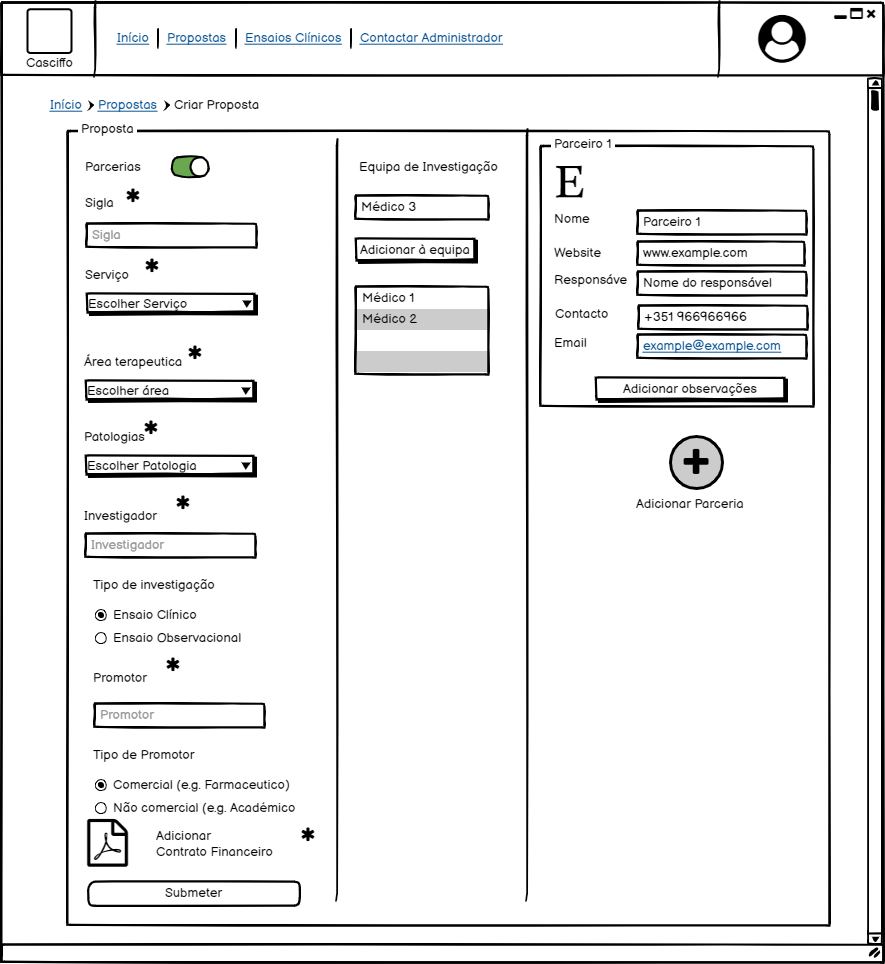
\includegraphics[scale=0.35]{Chapters/img/propostas/criar-proposta.png}
    \caption{Mock creation of a clinical investigation proposal.}
    \label{fig:criar-proposta}
\end{figure}

\subsection{Access control based on different user profiles}
\label{subsec:access-control-based-user-profiles}
The access control within the CASCIFFO application is based on roles.
As described in section 1, there are defined roles for each type of user.  
A user with the role `\acrshort{uic}` can manage their own clinical investigation, being able to edit and have a hand in advancing the state. In addition, it also has an overview over all ongoing investigations, not being able to edit those that weren't created by said user. Once this user logs in, a dashboard showing overall statistics of the platform, \textit{i.e.} number of active clinical trials, number of submitted proposals, etc.
The role `Financial` is responsible for validating and updating the financial components of the investigations, hence when a user with this role logs in, an appropriate financial management screen will be displayed, whereas the `Juridical` component validates the juridical component.  
The role `CA` is responsible for giving the final decision in whether an investigation proposal can have the go-ahead to begin their clinical trials or observations.  
A user of role `CA` once logged in, will be shown a primary screen displaying the overview of clinical investigation proposals awaiting validation.
Finally, we have the `Superuser` role, which besides having the ability to execute every mentioned action, it can also create new types of services, therapeutic areas and pathologies.


\subsection{Access by computer, tablet or smartphone}
\label{subsec:access-by-mobile-device}
CASCIFFO is a web-application which can be accessed via any device or browser. CASCIFFO offers an extended functionality to browsers that support service workers, since it utilizes the Progressive Web Application (PWA) framework, allowing it to be installed and used as an application.
Among the features a PWA allows, the framework was chosen by its ability to let an application run in offline-mode and versatility in that it can be installed via the browser, and used in similarity to a standalone mobile app. 

\subsection{Ability to export information in numerical or graphical mode}
\label{subsec:ability-to-export-info}
CASCIFFO offers the ability to export information via excel, and visualize graphic data within the app.  
There is a feature, shown in figure~\ref{fig:proposta-export-excel} that allows a user to export data, \textit{e.g.} a selected number of clinical investigation proposals. This feature is present in the screens showing listed data, \textit{e.g.} list of clinical investigation proposals, and the details of each clinical investigation, proposal or trial.

\begin{figure}[H]
    \centering
    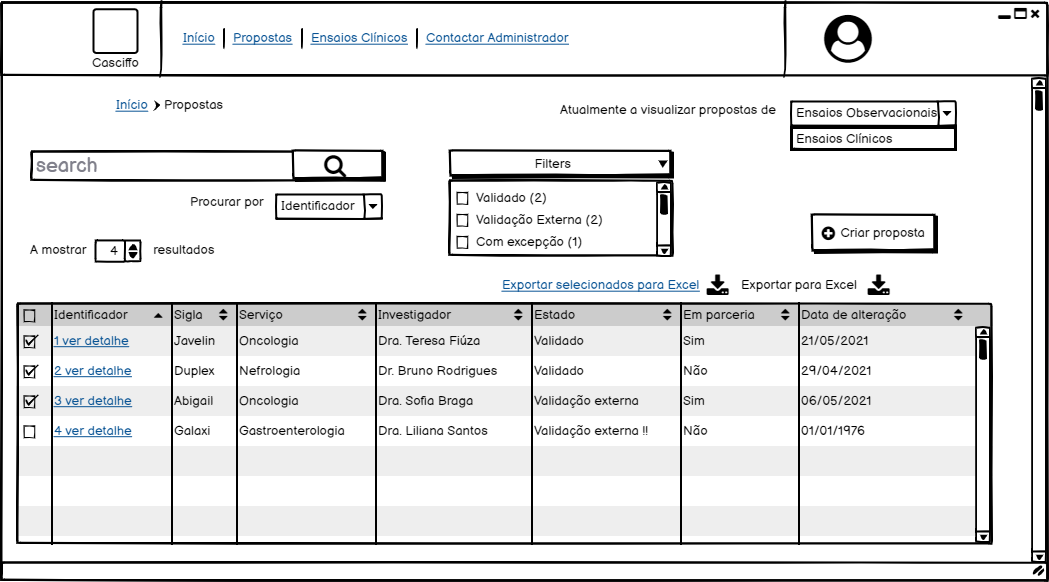
\includegraphics[scale=0.35]{Chapters/img/propostas/propostas-exportar-para-excel.png}
    \caption{Mock screen selecting clinical proposals to export into excel.}
    \label{fig:proposta-export-excel}
\end{figure}

\subsection{Ability to customize the form of visualization}
\label{subsec:ability-to-customize-visualization}
The ability to customize the form of visualization will be available in the initial screen of the app, the Dashboard, where the user will be able to view different types of graphs showing statistics based on the states of clinical investigations.


\section{Clinical Component Features}
The clinical component features of CASCIFFO consist in the following:
\begin{itemize}
    \item View detailed characteristics and evolution of clinical trials including the tested medicine or technique in question;
    \item Monitoring the set of patients included in clinical trials and their characteristics;
    \item Insertion of patient data in face-to-face or tele-consultation;
    \item Characteristics of the treatment associated with the clinical trial;
    \item Monitoring of the patient’s behavior under trial and its attendance;
    \item Monitoring of physical and financial assets;
    \item Monitoring of visits \& recording of adverse events.
\end{itemize}
In this section, all of the mentioned features will be detailed along with the visualization of a mock \acrshort{ui}.

\subsection{View detailed Characteristics and evolution of clinical Trials including the tested medicine or technique in question}
\label{subsec:clinical-investigation-details}
To view detailed information about a clinical investigation, one needs to first overview the clinical investigations and then click on the details of a desired clinical investigation. Considering this option, the user will be redirected to a screen detailing the study.  
The evolution of any clinical investigation consists of its proposal followed the trial activity once the proposal has been fully validated.
In figure~\ref{fig:proposta-detalhe}, the details of a clinical trial proposal can be viewed. The flow of state of a proposal is shown in the form of a bar in a straight forward manner. Each state corresponds to a division, box, in the bar and has three properties: the name of the State; the date it was completed in, if the state has otherwise not been completed, then a sequence of dashes will appear in its place; the deadline at which it should be completed and finally the entity responsible for advancing the state.  
It is possible to click in the box of a state to display information about the events that occurred during the time the proposal was in that state. 

\begin{figure}[H]
    \centering
    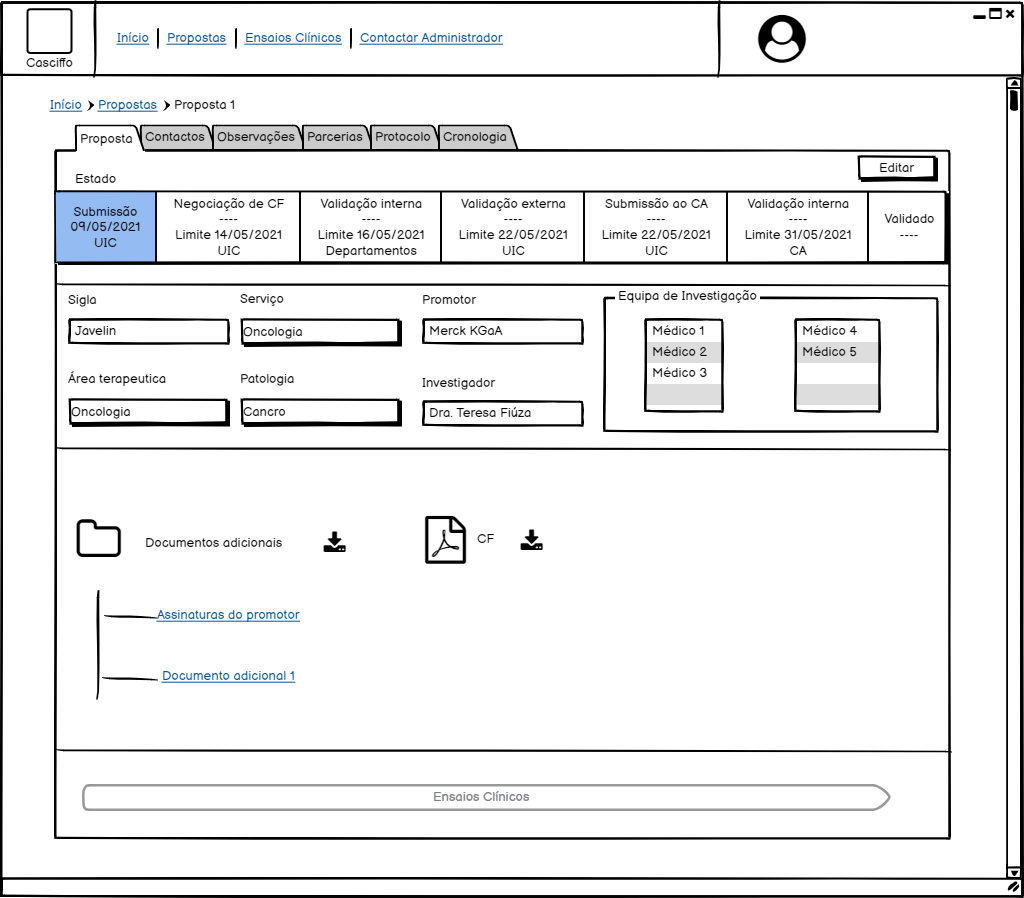
\includegraphics[scale=0.35]{Chapters/img/propostas/proposta-detalhe.png}
    \caption{Mock overview of a clinical investigation proposal.}
    \label{fig:proposta-detalhe}
\end{figure}

A clinical trial proposal considers five components alongside its principal details displayed as tabs and listed below: 
\begin{itemize}
    \item the Contacts ("Contactos") tab which corresponds to comments related to external communications, viewed in figure~\ref{fig:proposta-contactos};
    \item the Observations ("Observações") tab which contains comments made in regard to the proposal, viewed in figure~\ref{fig:proposta-observações};
    \item the Partnerships ("Parcerias") tab, where one can find the partnerships involved in the study proposal, viewed in figure~\ref{fig:proposta-parcerias};
    \item the validation Protocol ("Protocolo") tab, where it can be viewed the current state of affairs of the process described in section~\ref{subsec:visualization-clinical-trials-as-process}, and in figure~\ref{fig:proposta-protocolo};
    \item the Chronology ("Cronologia") tab that displays the timeline of events, as in figure~\ref{fig:proposta-cronologia}. Events include deadlines introduced by the user and the transition of states. The user will have the ability to specify the scope of the timeline, selecting the time range and type of events to view. 
\end{itemize}

All tabs, except the one pertaining to the Protocol validation, will have present the current state of the proposal.

\begin{figure}[H]
    \centering
    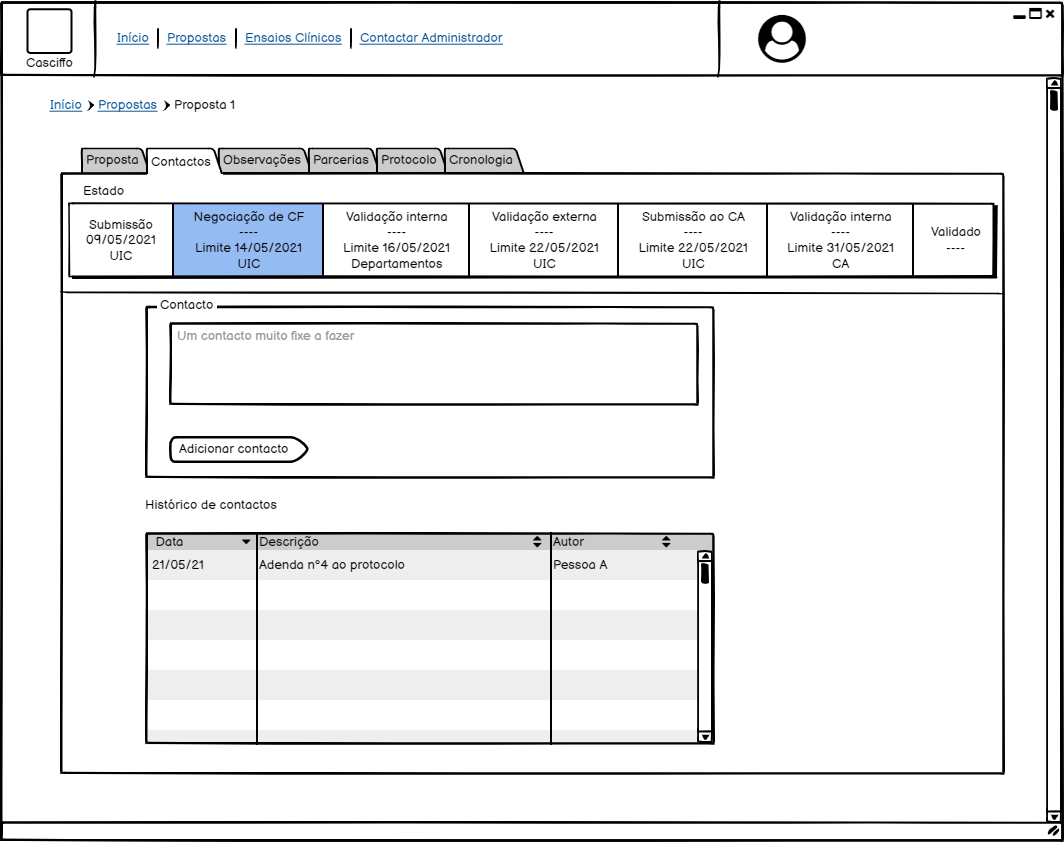
\includegraphics[scale=0.35]{Chapters/img/propostas/proposta-contactos.png}
    \caption{Mock overview of the contacts tab.}
    \label{fig:proposta-contactos}
\end{figure}

\begin{figure}[H]
    \centering
    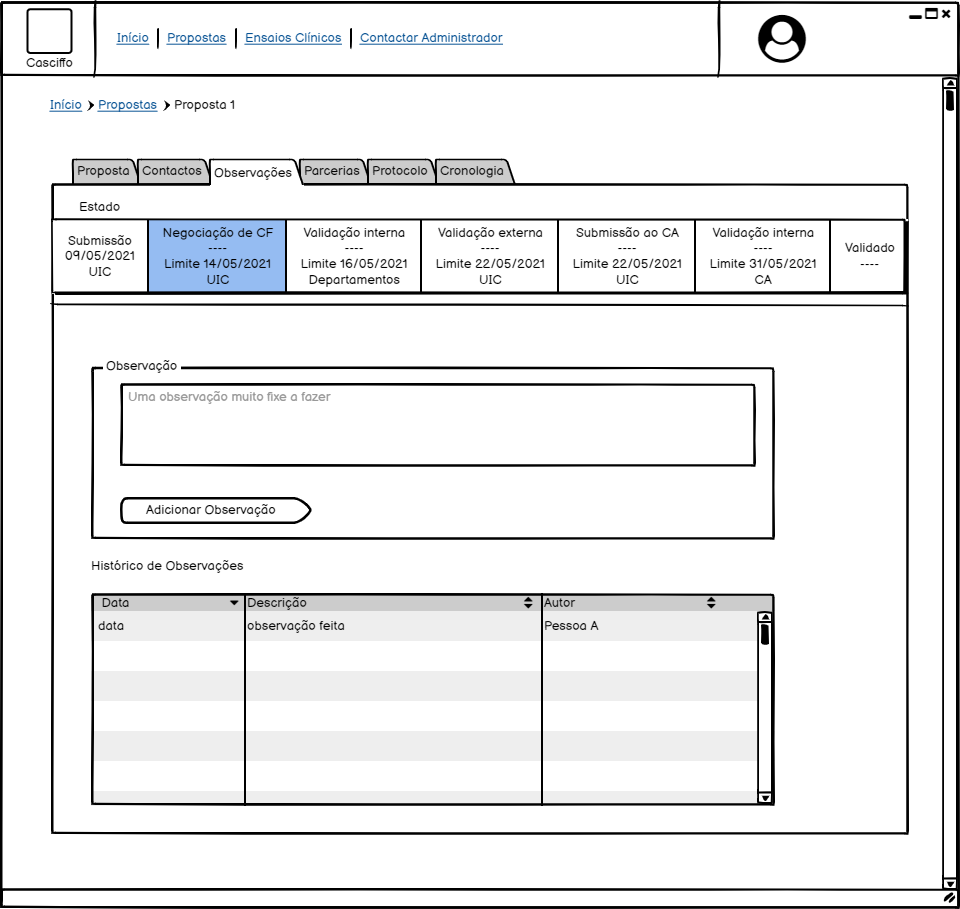
\includegraphics[scale=0.35]{Chapters/img/propostas/proposta-observações.png}
    \caption{Mock overview of the observations tab.}
    \label{fig:proposta-observações}
\end{figure}

\begin{figure}[H]
    \centering
    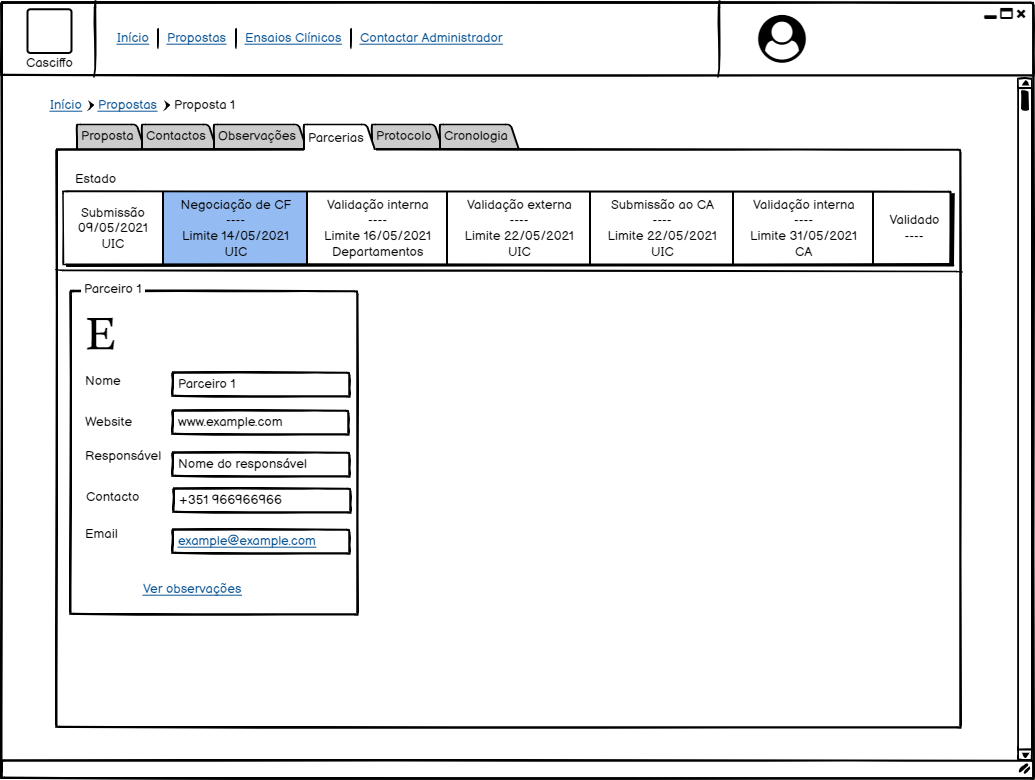
\includegraphics[scale=0.35]{Chapters/img/propostas/proposta-parcerias.png}
    \caption{Mock overview of the partnerships tab.}
    \label{fig:proposta-parcerias}
\end{figure}

\begin{figure}[H]
    \centering
    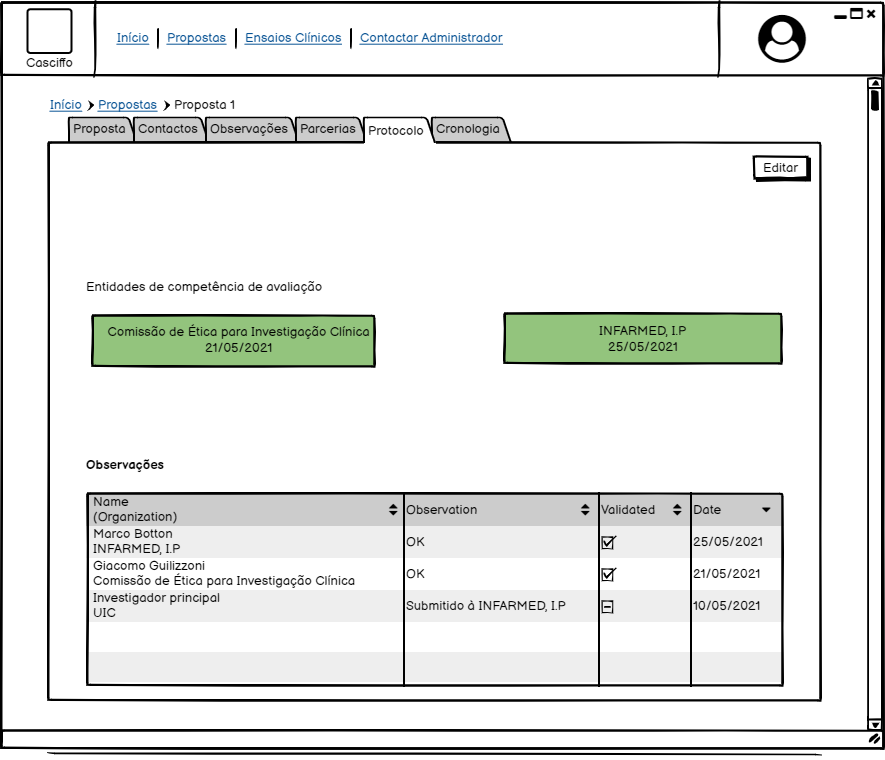
\includegraphics[scale=0.35]{Chapters/img/propostas/proposta-protocolo.png}
    \caption{Mock overview of the protocol tab.}
    \label{fig:proposta-protocolo}
\end{figure}

\begin{figure}[H]
    \centering
    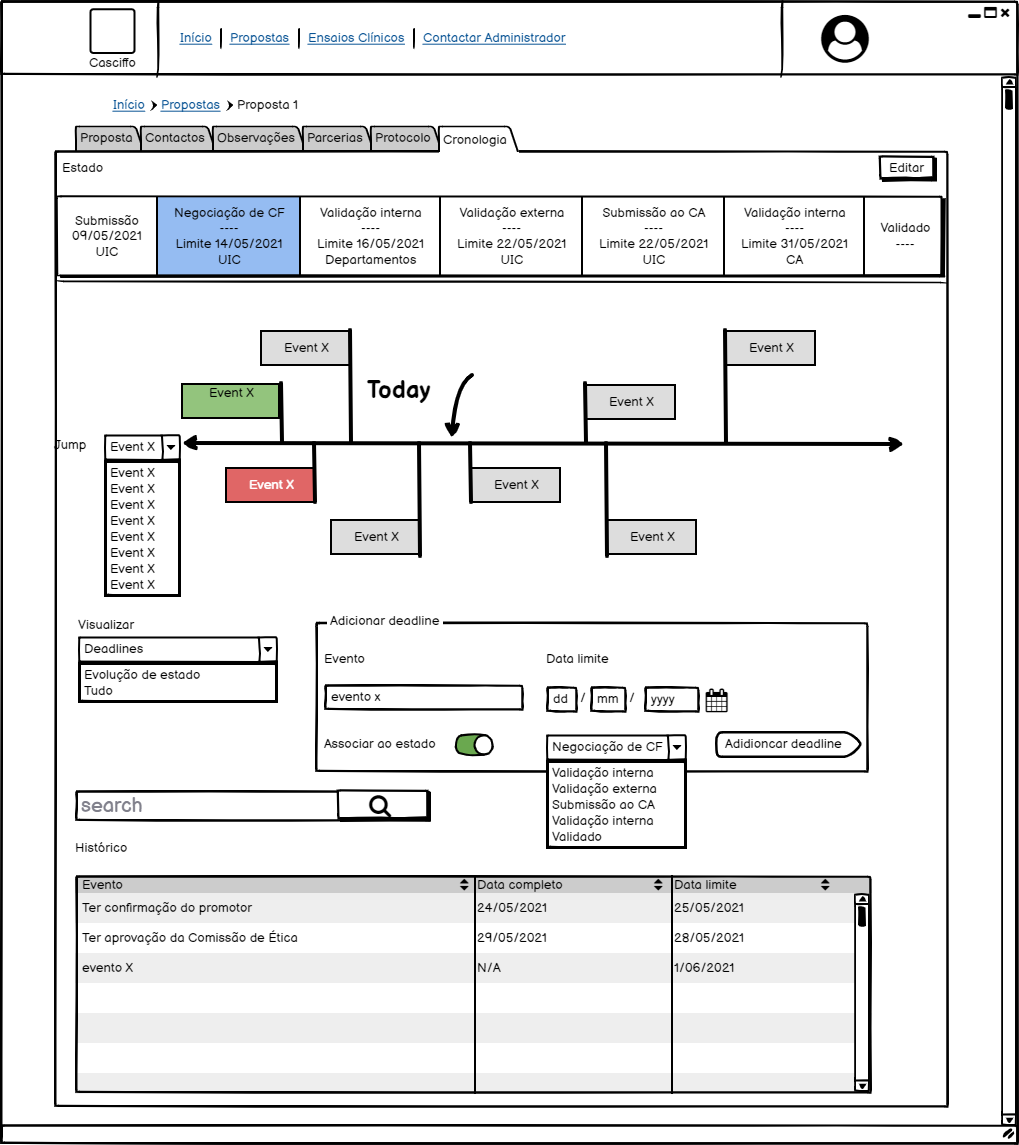
\includegraphics[scale=0.35]{Chapters/img/propostas/proposta-cronologia.png}
    \caption{Mock overview of the chronology tab.}
    \label{fig:proposta-cronologia}
\end{figure}



Once the proposal has reached its successful terminal state, as in section~\ref{subsec:clinical-investigation-proposals} a clinical trial will be created. To access the newly created trial, the user can either click the button "Ensaio Clínico" from the proposal details screen, as in figure~\ref{fig:proposta-detalhe}, or from the overview of clinical trials click on the details of one.  
In the screen dedicated to the clinical trial and presented in figure~\ref{fig:enasio-detalhe}, there are five different tabs: 
\begin{itemize}
    \item the clinical trial tab ("Ensaio Clínico") that displays the characteristics of the study;
    \item the scientific activities tab ("Atividades científicas"), viewed in figure~\ref{fig:ensaio-atividades-cientificas}, which includes scientific work in the scope of the study, such as articles, thesis, reports, etc.;
    \item  the visits tab ("Visitas") where the investigator team can have an overview of the history and scheduled visits;
    \item the patients tab ("Pacientes") with the purpose of showing an overview of the participants included in the trial;
    \item the partnerships tab ("Parcerias"), similar to the proposal's version of partnerships tab, displays the partnerships involved in the study;
    \item the financial management ("Financiamento"), where one can view the flow of monetary gain from visits and the partition between the investigator team.
\end{itemize}

\begin{figure}[H]
    \centering
    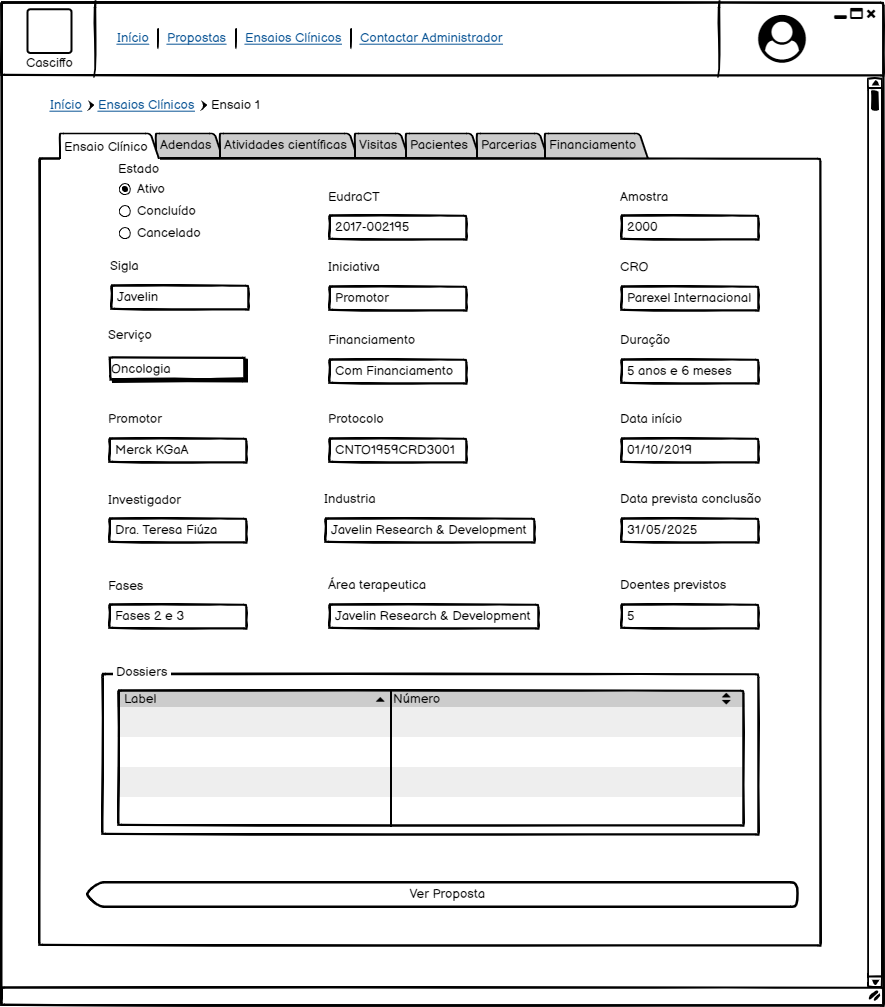
\includegraphics[scale=0.35]{Chapters/img/ensaios/ensaio-detalhe.png}
    \caption{Mock overview of the details of a clinical trial.}
    \label{fig:enasio-detalhe}
\end{figure}


\begin{figure}[H]
    \centering
    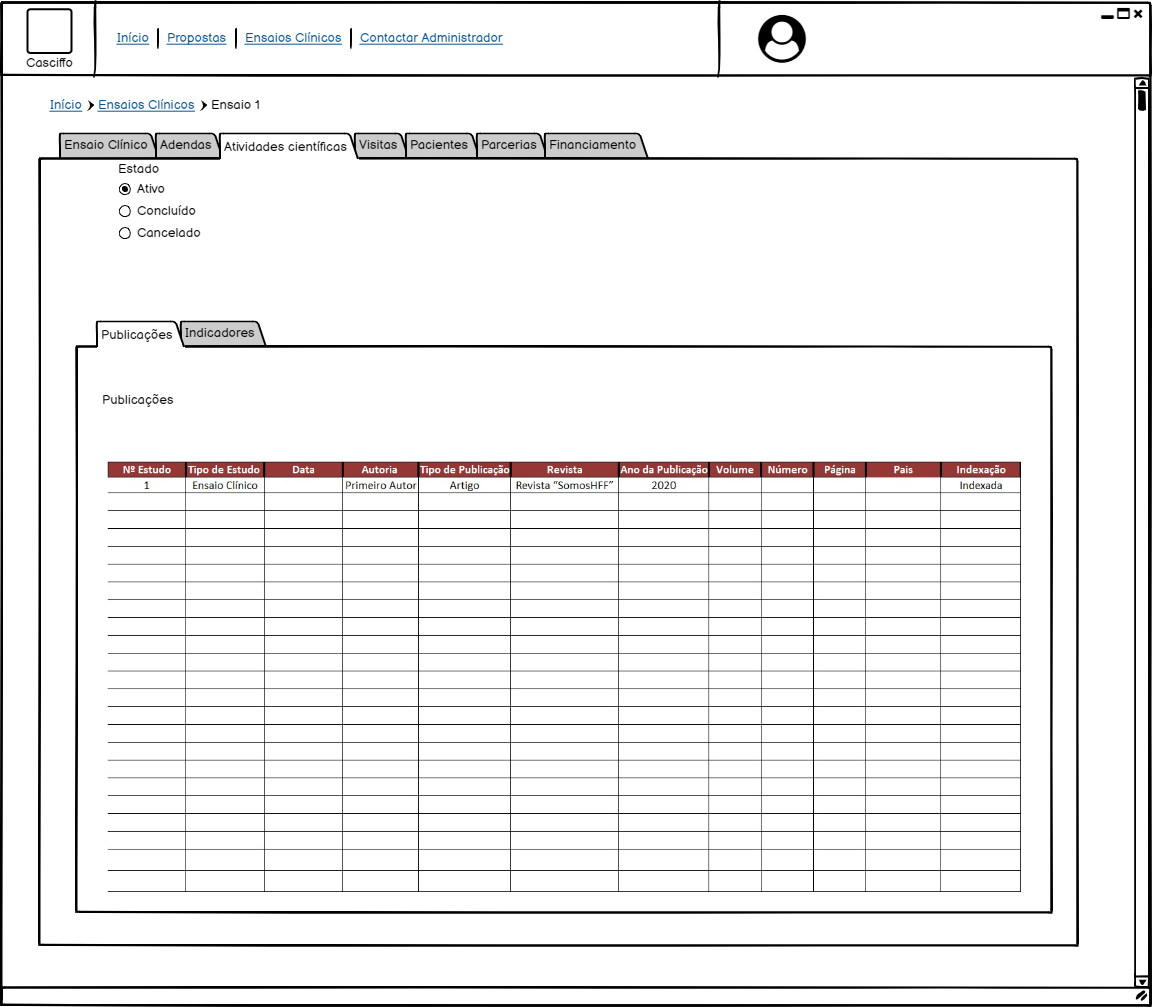
\includegraphics[scale=0.35]{Chapters/img/ensaios/ensaio-atividades-cientificas.png}
    \caption{Mock overview of scientific activities made within the scope of the investigation.}
    \label{fig:ensaio-atividades-cientificas}
\end{figure}


\subsection{Monitoring the set of patients included in clinical Trials and their characteristics}
\label{subsec:monitor-set-of-patients}
The details of the set of patients involved in a clinical trial will be displayed when viewing the details of said clinical trial, under the patients ("Pacientes") tab , illustrated in figure~\ref{fig:ensaio-participantes}. This tab displays the set of current participants undergoing the clinical trial and information such as the participant number, used to identify the participant throughout the study, the name of the participant, their age, the treatment branch they were assigned to within the scope of the study, their last and the closest upcoming visit.  
Included in this screen are the buttons Randomize ("Randomizar") and Add ("Adicionar").
The button "randomize" will randomly assign participants to treatment branches within the study, this one-time procedure is to be used once all the participants have been added to the clinical trial.
The button "add", will begin the procedure to add a patient. Upon clicking this button, the user will be shown a small box, as illustrated in figure~\ref{fig:ensaio-adicionar-paciente}, where he can input the name of the participant and then is also given the chance to immediately schedule several visits.

\begin{figure}[H]
    \centering
    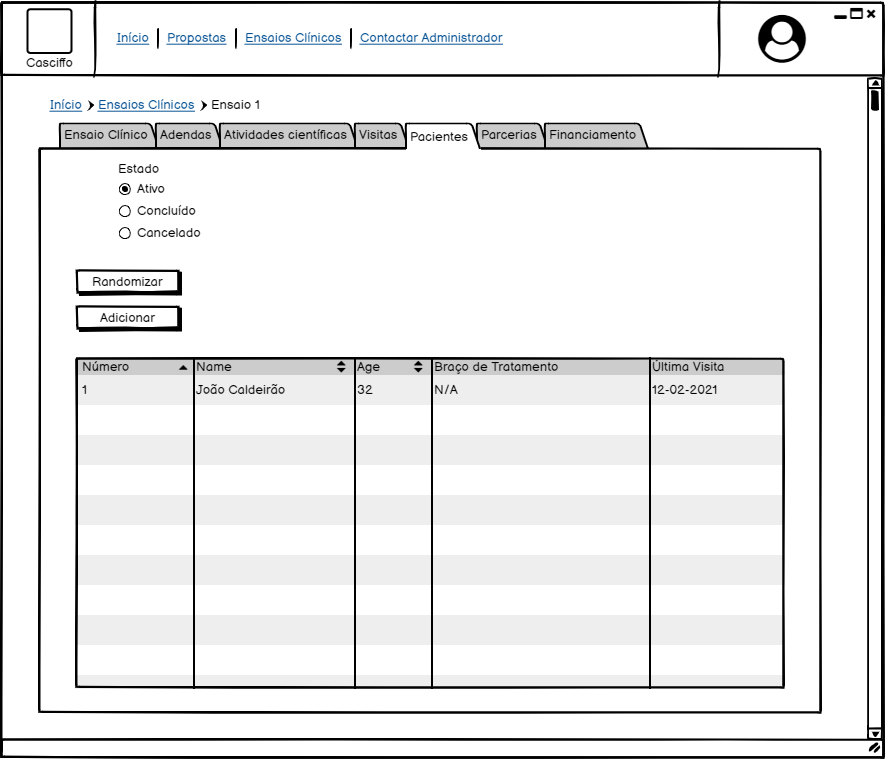
\includegraphics[scale=0.35]{Chapters/img/ensaios/ensaio-participantes.png}
    \caption{Mock overview of all participants included in the study.}
    \label{fig:ensaio-participantes}
\end{figure}

\begin{figure}[H]
    \centering
    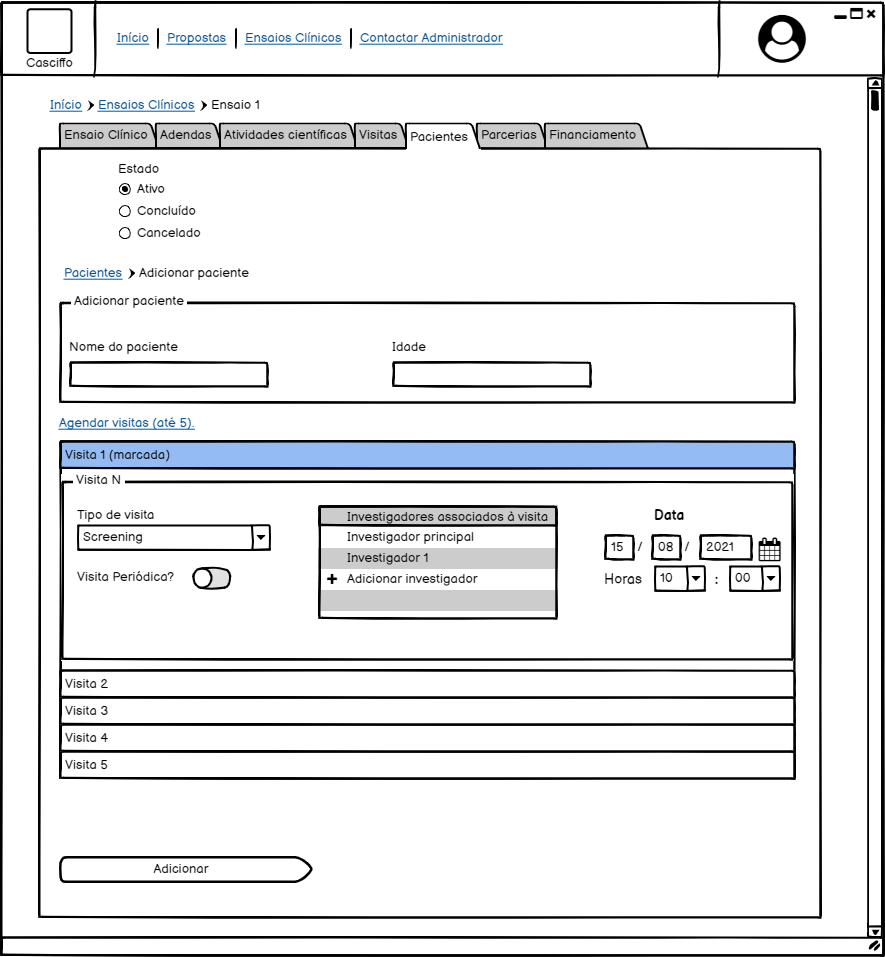
\includegraphics[scale=0.35]{Chapters/img/ensaios/ensaio-adicionar-paciente.png}
    \caption{Mock screen of adding a new patient as a participant in the study.}
    \label{fig:ensaio-adicionar-paciente}
\end{figure}

\subsection{Insertion of patient data in face-to-face or tele-consultation}

The insertion of patient data in the context of a visit is made by the investigator associated to the mentioned visit. In order to do this, the investigator has to navigate to the details of the visit, from the overview of clinical trials, to the details of the trial followed by the overview of visits and finally the details of the considered visit. Here the investigator can input observational data into the field "Observações" which will represent the observations made throughout the visit or tele-consultation. He is also asked to mark the attendance of the participant by clicking on a simple button "Marcar presença", as illustrated in figure~\ref{fig:ensaio-visita-detalhes}.

\begin{figure}[H]
    \centering
    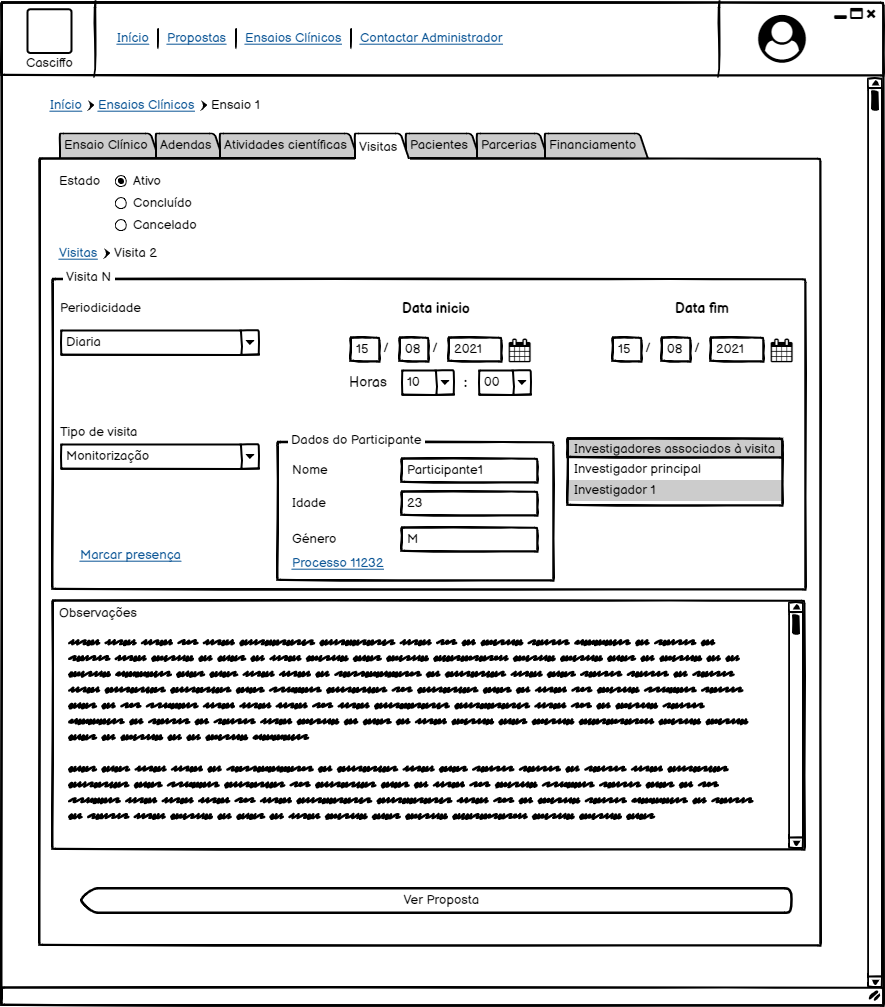
\includegraphics[scale=0.35]{Chapters/img/ensaios/ensaio-visita-detalhes.png}
    \caption{Mock overview of a visit's details.}
    \label{fig:ensaio-visita-detalhes}
\end{figure}


\subsection{Characteristics of the treatment associated with the clinical trial}
The characteristics of the treatment associated with clinical trials consists of three main factors, the service area it is within, the therapeutic field and the pathology the clinical trial aims to investigate/treat. These details can all be found in the detailed view of a clinical trial under the tab "Ensaio Clínico".  

\subsection{Monitoring of the patient’s behavior under trial and its attendance}
The monitoring of the patient's behavior and its attendance, can be tracked via the visits and in twofold. The first is to filter the visits, under the visits tab, to show only the visits related to the participant in question. The second is to view the details of this participant in particular, from the overview of total participants in the study, clicking on the details of the participant and then checking the tab "Attendance", as in figure~\ref{fig:ensaio-paciente-detalhes}. 

\begin{figure}[H]
    \centering
    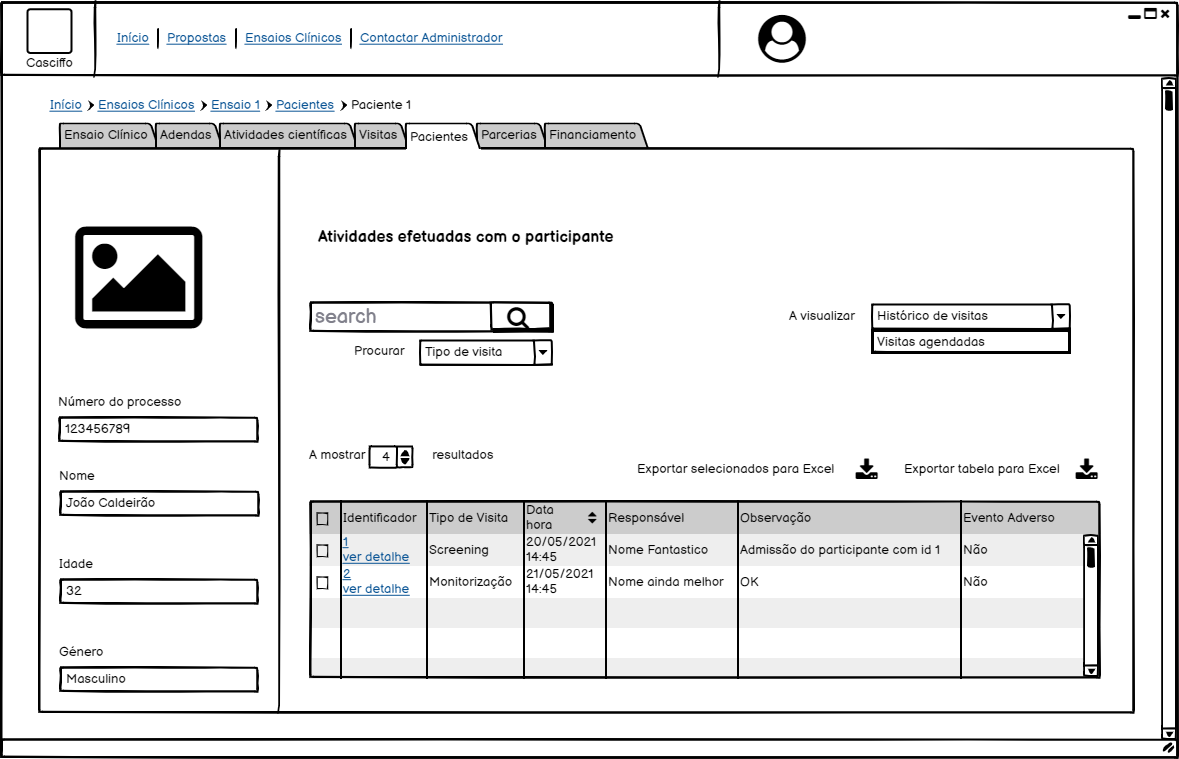
\includegraphics[scale=0.35]{Chapters/img/ensaios/ensaio-paciente-detalhes.png}
    \caption{Mock overview of patient details.}
    \label{fig:ensaio-paciente-detalhes}
\end{figure}

\subsection{Monitoring of physical and financial assets} 
In regard to the monitoring of physical assets, these can be viewed under the tab "Ensaio Clínico" while in the detail page of the clinical trial in question. The assets to be monitored are documentation archives, consisting of three fields: the Volume, a Label and the total Number.
CASCIFFO also offers another type of monitoring, the monetary flow. As described in section~\ref{subsec:clinical-trials}, each clinical trial has a financial management section that discriminates the earnings made by visit and the partitions of each team member involved in the study.  
Under the tab "Financiamento", the general monetary information, such as, total balance ("saldo"), amount per participant, etc., is displayed on a top section of the page. Below this section it can be observed another two tabs, differentiating the income made from the investigation team and the clinical trial itself. The first tab "EC", shown in figure~\ref{fig:ensaio-finance-ec}, shows the income made according to the visits done, whereas the second tab "Equipa", illustrated in figure~\ref{fig:ensaio-finance-team}, shows the income by team member.

\begin{figure}[H]
    \centering
    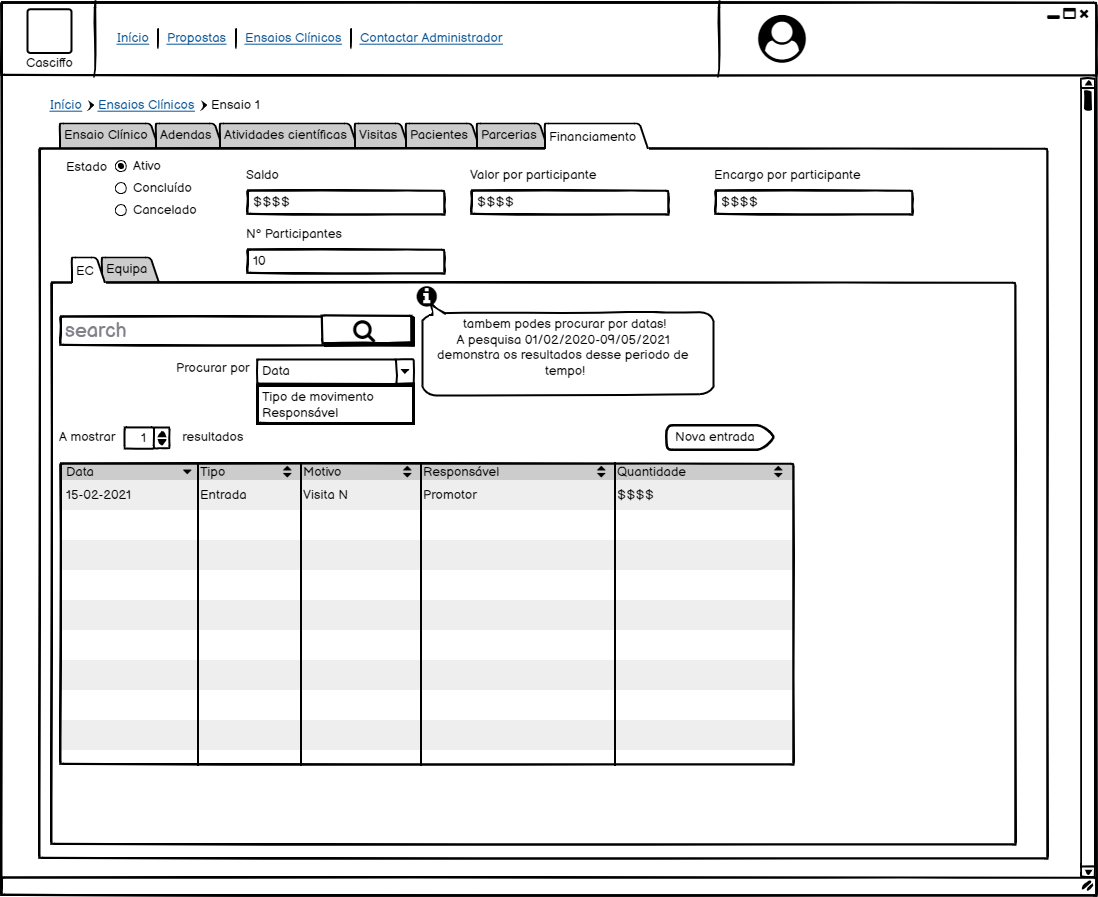
\includegraphics[scale=0.35]{Chapters/img/ensaios/ensaio-finance-ec.png}
    \caption{Mock detailed view of the income flow made in the investigation.}
    \label{fig:ensaio-finance-ec}
\end{figure}

\begin{figure}[H]
    \centering
    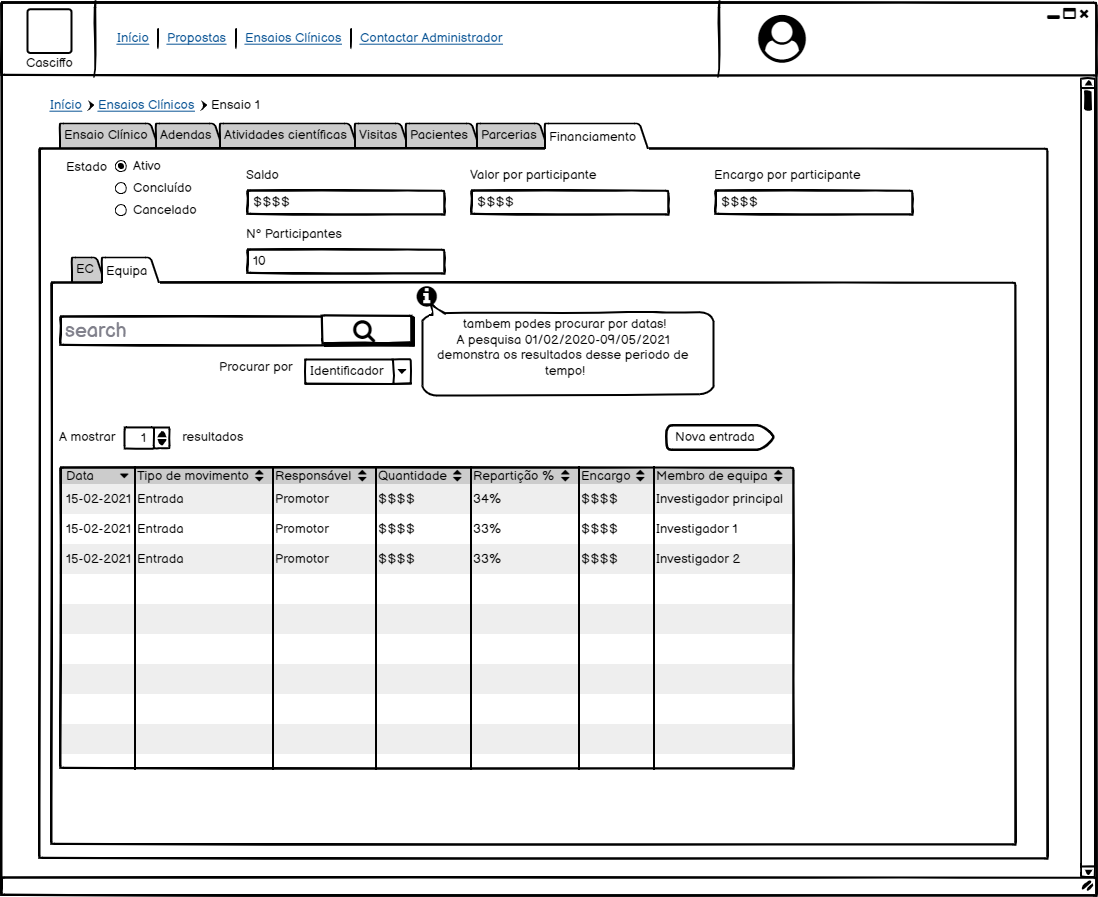
\includegraphics[scale=0.35]{Chapters/img/ensaios/ensaio-finance-team.png}
    \caption{Mock detailed view of income flow divided by the investigator team.}
    \label{fig:ensaio-finance-team}
\end{figure}

\subsection{Monitoring of visits \& recording of adverse events} 
The monitoring of visits during a clinical trial can be tracked and viewed under the tab "Visitas", in the detailed screen of a clinical trial.
In this setting, any investigator (associated to the clinical trial) is able to view and track the past and scheduled visits made by the team. However, only the investigators associated to a visit are able to manipulate them. When creating a visit, that visit will automatically be associated to its creator, giving also the option to associate other investigators to the same visit, allowing them to freely edit the visit details. Along with this option, the investigator is required to fill in the fields depicted in figure~\ref{fig:ensaio-visitas}. These fields are as follows: the periodicity ("Períodicidade") that can be turned ON in case the visit is a reoccurring one with the ability to schedule at a custom interval in days; the type of visit ("Tipo de visita"), that has three possible inputs, Screening, indicating the first visit, Monitoring ("Monitorização") indicating a motoring visit and finally a Closeout visit, which indicates the final visit done to a participant. In case the visit is periodic, the field of `end date` ("Data fim") becomes mandatory to fill.  

\begin{figure}[H]
    \centering
    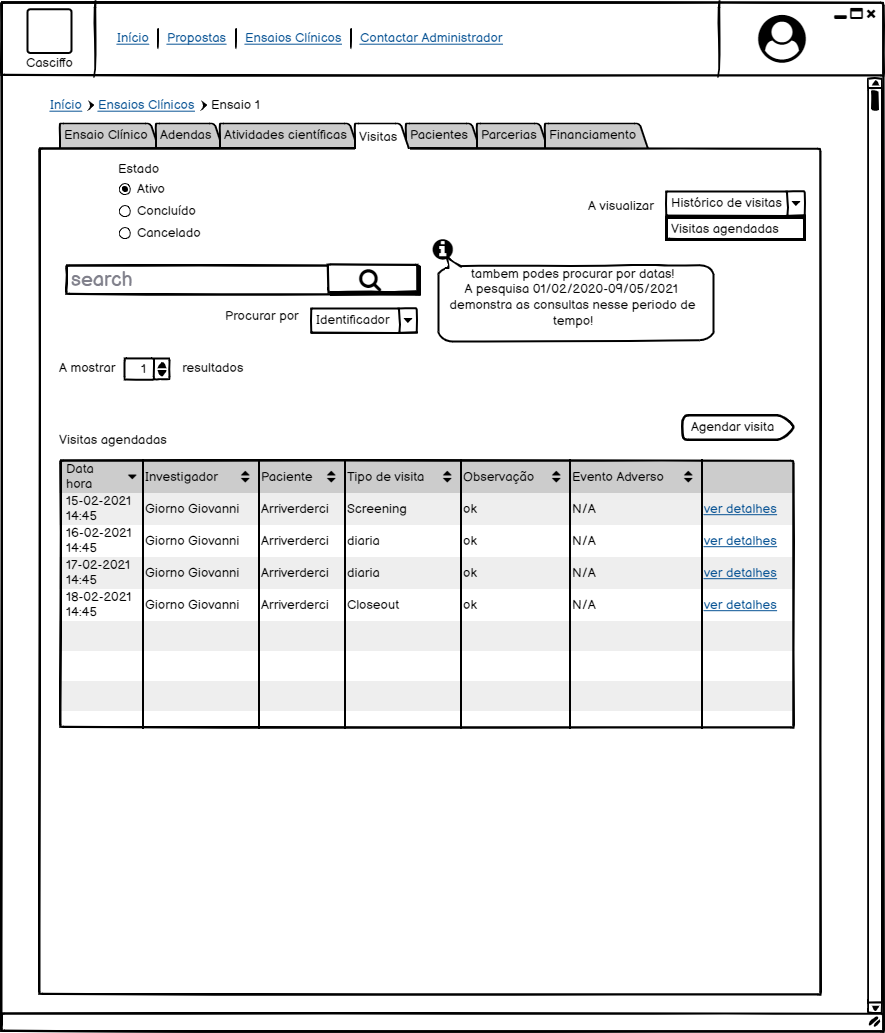
\includegraphics[scale=0.35]{Chapters/img/ensaios/ensaio-visitas.png}
    \caption{Mock overview of visits scheduled in the clinical trial.}
    \label{fig:ensaio-visitas}
\end{figure}

When a visit occurs, the associated investigators will have access to the observations ("Observações") field and adverse event ("Evento adverso") warning. In addition to this, the field "Marcar presença" is now available to mark attendance.

\section{Non-Functional Requirements}
METER AQUI TABELA COM REQUISITOS NAO FUNCIONAIS
NOTIFICAÇÕES/PAGINAÇÃO/ETC